\documentclass[twoside]{article}

% Language and font encodings
\usepackage[english]{babel}
\usepackage{amsmath}
\usepackage[a4paper,top=3cm,bottom=2cm,left=3cm,right=3cm,marginparwidth=1.75cm]{geometry}
\usepackage{graphicx}
\usepackage{tabularx}
\usepackage{natbib}
\usepackage[colorinlistoftodos]{todonotes}
\usepackage[colorlinks=true, allcolors=blue]{hyperref}
\usepackage{wrapfig}
\DeclareMathAlphabet{\pazocal}{OMS}{zplm}{m}{n}
\usepackage{setspace}
\usepackage{hyperref}
\hypersetup{
    colorlinks=true,
    linkcolor=blue,
    filecolor=magenta,      
    urlcolor=cyan,
}
\urlstyle{same}

%%%%%%%%%%%%%%%%%%%%%%%%%%%%%%%%%%%%%%%%%%%%%%%%%%%%%%%%%%%%%%%%%%%%%%%%%%%%%%%%

\begin{document}

\begin{center}
  {\Large \bf Milestone 2: Recombination History of the Universe.}\\[4ex]
  {\large Daniel Herman}\\[4ex]
  \normalsize
  \today
  \vspace*{2ex}
      
  \begin{minipage}[t]{12cm}
      
  {\bf Abstract.} Calculating the evolution of baryonic recombination, ionization, and the optical depth of the universe.
	
  \vspace*{2ex}
  \end{minipage}

\end{center}

\section{Introduction}\label{sec:intro}

In this report we continue working towards simulating the Cosmic Microwave Background (CMB). We calculate the ionization fraction of hydrogen in the early universe and use this information to calculate the optical depth of the universe as a function of time. The optical depth is then used to create a visibility function, which is a probability distribution showing the probability that a primordial photon scatters for the last time off of electrons and escapes into open space.\\

Again, a skeleton code was provided to outline the goals and steps needed to complete Milestone 2. All calculations were made using FORTRAN 90, and the plotting was done using Python. The code can be found at \url{https://github.com/hermda02/CosmologyII}.

\section{Equations}\label{sec:eq}

The same notation from Milestone 1 is used here as well, namely
\begin{equation}
a(t) = \dfrac{a_0}{1+z} \Rightarrow z = \dfrac{a_0}{a} -1
\end{equation}
\begin{equation}
x = \ln(a)
\end{equation}
\begin{equation}
H = \dfrac{\dot{a}}{a} = H_0\sqrt{(\Omega_b + \Omega_m)a^{-3} + (\Omega_r + \Omega_{\nu})a^{-4} + \Omega_{\Lambda}}
\end{equation}
\begin{equation}
\dfrac{d\eta}{dt} = \dfrac{c}{a}
\end{equation}


Other equations used in the project can be found in Callin (2006). Only the general equations will be presented in this report.

The first quantity which we calculate is the electron density $n_e$. We utilize the fractional electron density $X_e \equiv n_e/n_H$ where $n_H$ is the hydrogen density. Since the mass of the proton is far larger than the electrons, and we assume that no heavier elements such as helium are present, we define 

\begin{equation}
n_H \simeq n_p = n_b \approx \dfrac{\rho_b}{m_H} = \dfrac{\Omega_b \rho_c}{m_Ha^3}
\end{equation}

\noindent where $n_p$ is the proton density and $\rho_c \equiv \dfrac{3 H_0^2}{8 \pi G}$ is the critical density of the universe. We utilize the assumption that $T_b = T_r = T_0/a = 2.725{\rm K}/a$ during our \mbox{calculations}. Finally, we use the fact that $n_H = n_b$ to define the electron density as
\begin{equation}\label{eq:elecdense}
n_e \equiv X_e n_b.
\end{equation}

\subsection{Fractional Electron Density}\label{sec:elecfrac}
We have two different equations for the fractional electron density: the Saha and the Peebles equations. The Saha equation is valid for large fractional electron densities, which we define to be $X_e > 0.99$. When $X_e < 0.99$, we use the Peebles equation.\\

\noindent The Saha equation is defined as
\begin{equation}\label{eq:saha}
\dfrac{X_e^2}{1-X_e} = \dfrac{1}{n_b}\Big(\dfrac{m_ek_BT_b}{2\pi\hbar^2}\Big)^{3/2}e^{-\epsilon_0/k_BT_b}
\end{equation}

\noindent where $T_b$ is the baryon temperature of the universe, and $\epsilon_0$ is the ionization energy of hydrogen. We use the Peebles equation for lower values of $X_e$ because it gives a more accurate approximation,

\begin{equation}\label{eq:peeble}
\dfrac{dX_e}{dx} = \dfrac{C_r(T_b)}{H}\Big[\beta(T_b)(1-X_e) - n_H\alpha^{(2)}(T_b)X_e^2\Big]
\end{equation}

\noindent where

\begin{align}
C_r(T_b) &= \dfrac{\Lambda_{2s \rightarrow 1s}+\Lambda_{\alpha}}{\Lambda_{2s \rightarrow 1s}+\Lambda_{\alpha}+\beta^{(2)}(T_b)}\\
\Lambda_{2s \rightarrow 1s} &= 8.227s^{-1}\\
\Lambda_{\alpha} &= H\dfrac{(3\epsilon_0)^3}{(8 \pi)^2 n_{1s}}\\
n_{1s} &= (1-X_e)n_H\\
\beta^{(2)}(T_b) &= \beta(T_b)e^{3\epsilon_0/4k_BT_b}\\
\beta(T_b) &= \alpha^{(2)}(T_b)\Big(\dfrac{m_ek_BT_b}{2\pi\hbar^2}\Big)^{3/2}e^{-\epsilon_0/k_BT_b}\\
\alpha^{(2)}(T_b) &= \dfrac{64 \pi}{\sqrt{27 \pi}}\dfrac{\alpha^2}{m_e^2}\dfrac{\hbar^3}{c}\sqrt{\dfrac{\epsilon_0}{k_B T_b}} \phi_2(T_b)\\
\phi_2(T_b) &= 0.448 \ln (\epsilon_0/k_BT_b). 
\end{align}

The above equations are used to describe the atomic physics at work here. Peebles' equation takes into account the transition rates between the ground state and the first excited state of the hydrogen atom. Other states and atoms are neglected in this equation for simplification. We see that the Peebles' equation is a straight forward first-order linear equation which is simple to solve.\\

\subsection{Optical Depth and Visibility Function}\label{sec:optic}

The optical depth is defined as
\begin{align}\label{eq:depth}
\tau(\eta) &= \int_{\eta}^{\eta_0} n_e \sigma_Tad\eta'\\
\tau(a) &= \int_a^{a_0} \dfrac{n_e \sigma_T c}{H(a)}da'
\end{align}
which denotes the probability that a photon scatters off of an electron. We see that $\tau$ is directly dependent on the electron density $n_e$ and the Thomson cross-section $\sigma_T$. Another useful optical depth equation follows directly from \ref{eq:depth}
\begin{equation}\label{eq:depthderiv}
\tau' = -\dfrac{n_e\sigma_Ta}{\pazocal{H}}.
\end{equation}

The last equation which we will use in this part of the project is a probability distribution function called the visibility function,

\begin{align}\label{eq:vis}
g(\eta) &= -\dot{\tau}e^{-\tau(\eta)} = -\pazocal{H}\tau'e^{-\tau(x)} = g(x)\\
\tilde{g}(x) &= -\tau'e^{-\tau} = \dfrac{g(x)}{\pazocal{H}}\\ 
\int_0^{\eta_0}g(\eta)d\eta &= \int_{-\infty}^0 \tilde{g}(x)dx = 1.
\end{align}
The visibility function describes the probability density for a photon to scatter at time $x$. 

\clearpage

\section{Implementation}\label{sec:imp}

As in Milestone 1, we utilize FORTRAN90 and the skeleton code provided to complete this project. The same initial conditions are used here again to keep each module consistent. We initialize $a$ with $a_{rec} = 10^{-10}$, and $a_0 = 1$ (today). Furthermore, we initialize the fractional electron density $X_e$ with $X_e(a_{rec}) = 1$, as we set $\tau_0 = 0.$ Again, arrays for the time variables $a$, $z$ and $\eta$ are initialized for calculations.

\subsection{Fractional Electron Density}\label{sec:fraccalc}
Since we assume that $X_e = 1$ initially, we begin solving for the fractional electron density as a function of time using the Saha equation (eq.\ref{eq:saha}). We solve for $X_e$ as a function of $a$ using the assumptions presented in section \ref{sec:eq}, namely $T_b(a) \propto a^{-1}$ and $n_b \propto a^{-3}$. When $X_e < 0.99$, we switch to the Peebles' equation (eq. \ref{eq:peeble}). Since the Peebles' equation is a first order differential equation, we utilize the ODE solver utilized in Milestone 1. A subroutine was written to solve for the differential steps utilized by the ODE solver. At large redshift (small $a$), $T_b$ approaches large values, which causes computational issues particularly in the calculation of $\beta^{(2)}$ as we are taking the product of two very small numbers. In order to avoid this issue, we set $\beta^{(2)} = 0$ when $T_b \geq 169K$. This value was determined through trial and error. The evolution of the fractional electron density is seen in figure \ref{fig:elecfrac}. With values for $X_e$, we can determine the electron density of the universe using the relation in equation \ref{eq:elecdense}.\\

To verify that the electron density evolution is smooth for all arbitrary values of $a$ and $x$, we utilize a spline function which is has also been provided in the code. To make sure that resolution isn't lost, we spline $\log(n_e)$.

\subsection{Optical Depth}\label{sec:optcalc}

Next we calculate the optical depth of the universe using equation \ref{eq:depth}. The ODE solver is used again to aid in solving for the optical depth. Again, a subroutine is used to solve for the differentials. The first and second derivatives of the optical depth are also solved for to allow us to visualize how the optical depth changes over time. The first derivative, $\tau'$ is solved for directly using equation \ref{eq:depthderiv}, and the second derivative is solved using the spline function. The optical depth (and its derivatives) are splined in the same way as the electron density as mentioned in section \ref{sec:fraccalc}.


\subsection{Visbility Function}\label{sec:viscalc}

Finally, we can solve for the visibility function using the equations in section \ref{sec:optic}. Unlike the previous calculations, we can solve for $g(x)$ directly using the values of $\tau$ and $\tau'$ found in the previous section. The derivatives of the visibility function are also computed to visualize the functions behavior. As above, $g'(x) = -\tau''(x)e^{-\tau(x)}+\tau'^2(x)e^{-\tau(x)}$ can be solved for directly using the derivatives of $\tau$, and $g''(x)$ is computed using the spline function.

\clearpage

\section{Results}\label{sec:results}

As per request, the fractional electron density as a function of redshift is shown below. As we hoped, the calculations of $X_e$ yield a smooth, continuous function. We see that the density begins to quickly drop right before recombination ($z = 1100$). As redshift increases, the expansion rate of the universe causes the fractional electron density to decrease quickly. This is expected since the baryon density decreases proportional to $a^{-3}$. It is important to make the y-axis logarithmic to study the behavior, as $X_e$ quickly drops below 0.1. The fractional electron density continues to decrease up to today, however the rate of change begins to decrease at around $z=800$.

\begin{figure}[ht!]\label{fig:elecfrac}
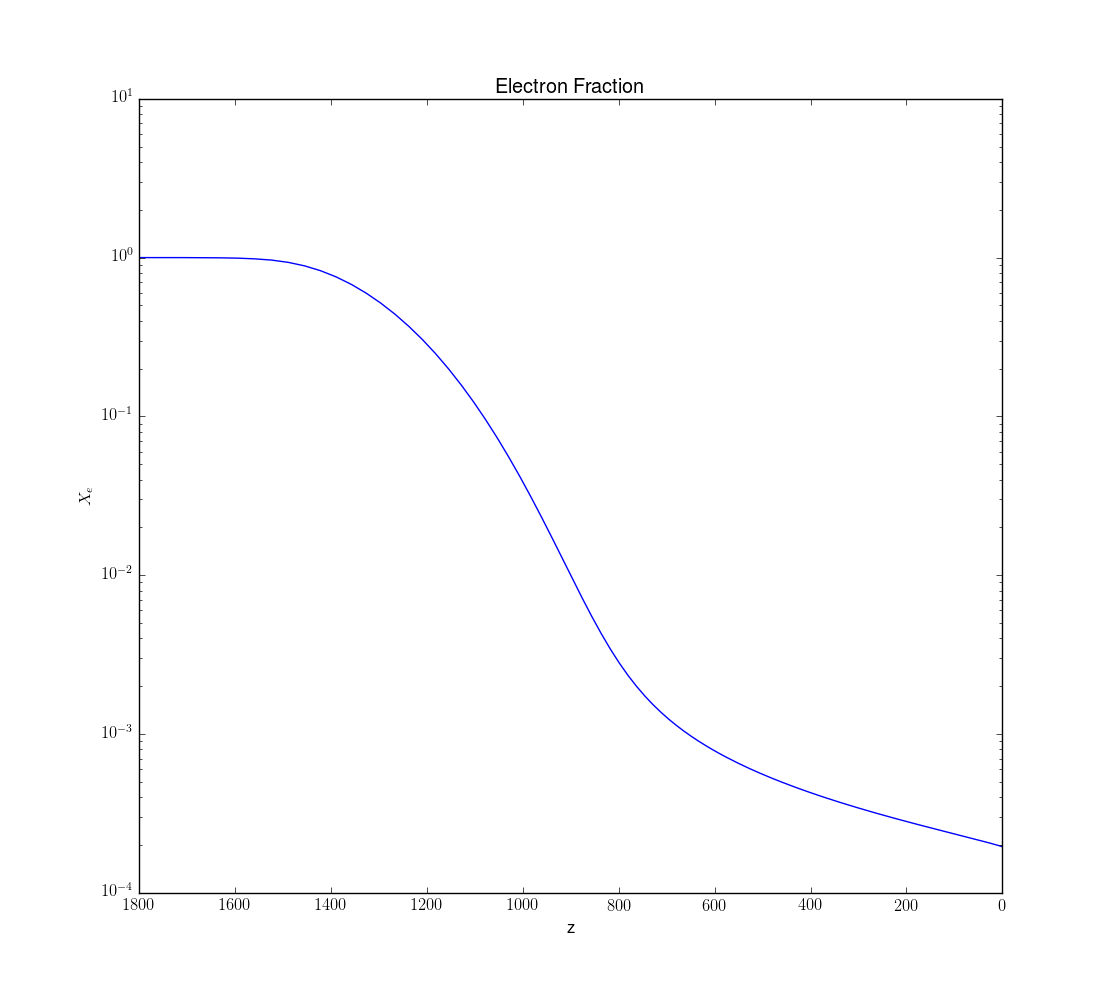
\includegraphics[scale=0.45]{electronfraction}
\caption{The electron fraction as a function of redshift.}
\end{figure}

\clearpage

The optical depth is shown below as a function of $x=log(a)$. As expected, the optical depth follows the electron density. Photons are unable to escape the dense universe until around $x = -7$, when the optical depth reaches $\tau = 1$. We expect this to be the time at which the last scattering of the primordial photons to occur. Again, the calculations of $\tau$ and its derivatives provide smooth, continuous functions.

\begin{figure}[ht!]\label{fig:optdepth}
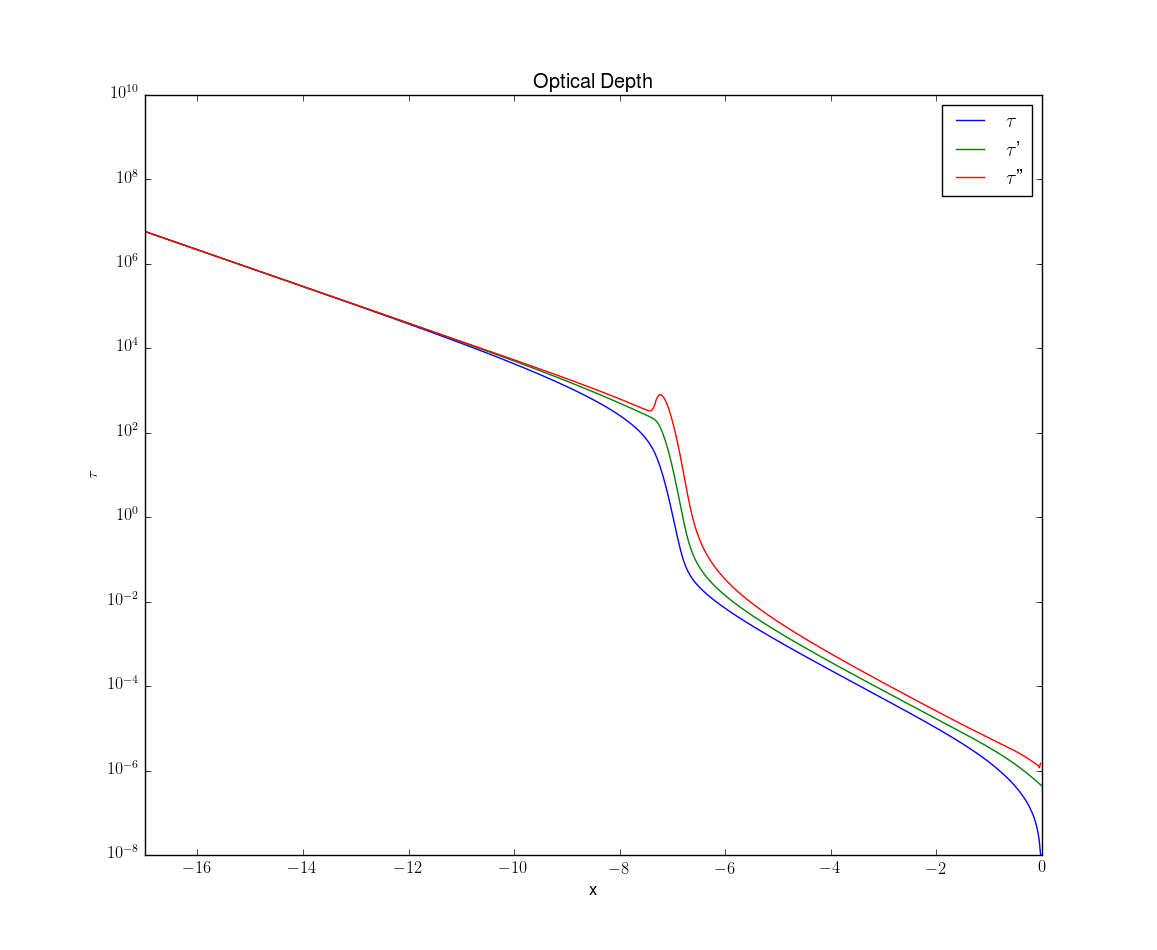
\includegraphics[scale=0.5]{opticaldepths_nolog}
\end{figure}

\clearpage

The visibility function helps to visualize the probability of when a photon scatters for the last time. We only concern ourselves with the chunk of time around $x=-7$, becuase at smaller scale factors the universe is too dense for last scattering to occur, and at larger scale factors all of the photons will have alread scattered. Calculating for $g(x)$ yields a smooth, asymmetrical probability distribution which, as predicted above, has a peak around $x=-7$. All of the primordial photons scatter for the last time between redshifts $z=700-1400$ where the temperature variation is within a few thousand $K$.

\begin{figure}[ht!]\label{fig:vis}
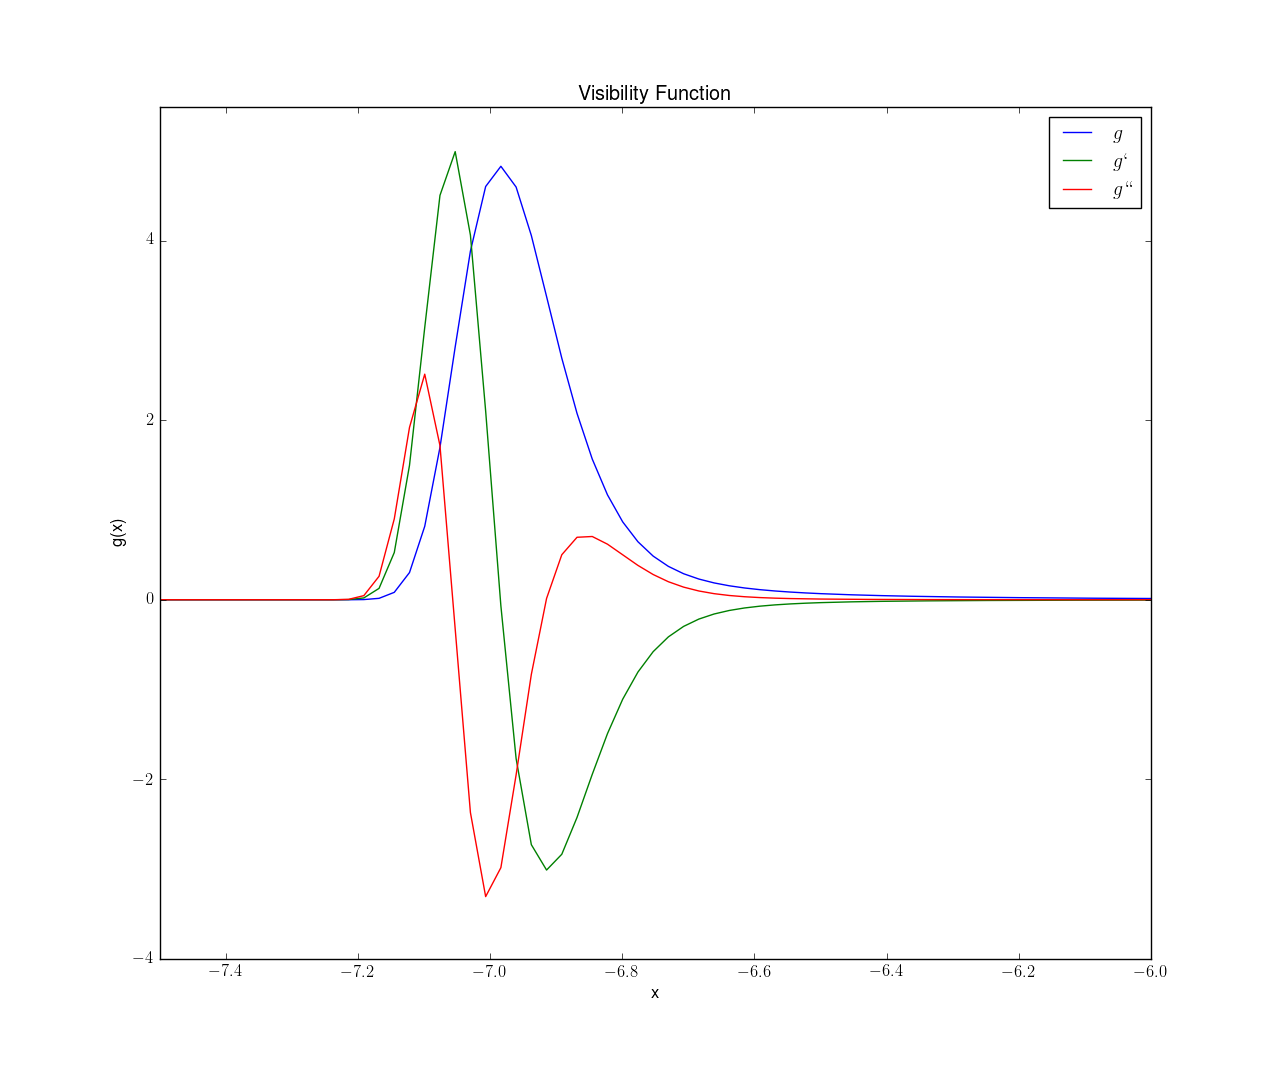
\includegraphics[scale=0.45]{visibilityfunctions}
\end{figure}


\section{Conclusion}\label{sec:conc}

The calculations required for Milestone 2 were successfully completed and produced the expected results. Some easy to fix numerical precision issues were encountered, and functions solving for electron density, optical depth, and visibility function values were created for utilization in further milestones. The physical concepts used in this milestone were easy to implement with the help of the ODE solver and the spline technique.

\end{document}